\documentclass[10pt,twocolumn,letterpaper]{article}
\usepackage{cvpr}
\usepackage{times}
\usepackage{graphicx}
\usepackage{amsmath}
\usepackage{amssymb}
\usepackage{url}
\usepackage[pagebackref=true,breaklinks=true,colorlinks,bookmarks=false]{hyperref}

\def\GroupID{G27} % <------- ENTER YOUR GROUP ID HERE

\begin{document}
	\title{Time Series Forecast with Neural Networks}
	\author{Zijian Wang (\textit{40011864}) \and Matheus Nogueira (\textit{40220168})  }
	\maketitle
	
	\begin{abstract}
		This project aims to implement and compare various methods for Time Series Forecasting, since the classical ones, such as ARIMA and GARCH until Recurrence Neural Networks and Prophet. The goal is to evaluate if the later, and more complex methods, necessarily result in better forecasting, with respect to the \textit{RMSE} metric or if simpler methods are precise enough to be chosen for either stationary and non-stationary financial series.  
	\end{abstract}
	
	%------------------------------------------------------------------------
	\section{Introduction}
	
	Implementing precise models for Time Series Forecasting is crucial to various areas of knowledge, being fundamental to Financial Analysis of Stock Returns and Currency, which are types of time series chosen to be worked with. For that purpose, one could say that is a difficult task to chose between the huge amount of different methods, since each of them have its own advantages and disadvantages. For instance, simple linear models such as ARIMA are easy to understand and implement, but may be too simple and inflexible to model Stock Returns. On the other hand, MLPs and Recurrence Networks may present themselves with precise forecasts but with a complex theory behind and possible training difficulties may arise - over fitting is a classic example.
	
	With being said, this project's goal is to implement different time series methods for 3 financial time series, all them with a stationary and non-stationary form, so that one can compare the quality of each model prediction.
	
	%------------------------------------------------------------------------
	\section{Methodology \& Experimental Results}
	
	Three financial time series were chosen to be used in this project. All of them have weekly frequency with time period from 2010 to 2019 and can be found on \url{finance.yahoo.com/}. One of the series is the stock price of American Airlines while the two others are currency rates of American Dollars with Canadian Dollars and Brazilian Real:
	\begin{itemize}
		\item American Airlines Group Inc. (AAL)
		\item USD/CAD (CAD=X)
		\item USD/BRL (BRL=X)
	\end{itemize}
	
	Once the series are chosen, the first step of the methodology was to develop a Time Series Analysis procedure, in order to gain information about each of them. With this analysis the goal was to gather information regarding seasonality, stationarity, trend, missing values and the number of differentiation needed to obtain a stationary behaviour. The results of this analysis is expressed on the table below.
	
	\begin{table}[h]
		\centering
		\begin{tabular}{|l|c|c|c|c|}
			\hline
			& \multicolumn{1}{l|}{Trend} & \multicolumn{1}{l|}{Statio} & \multicolumn{1}{l|}{NumDiff} & \multicolumn{1}{l|}{Season} \\ \hline
			ALL     & Yes                        & No                              & 1                              & No                            \\ \hline
			USD/CAD & Yes                        & No                              & 1                              & No                            \\ \hline
			USD/BRL & Yes                        & No                              & 1                              & No                            \\ \hline
		\end{tabular}
	\end{table}
	
	In order to determine stationarity two methods were used: first, a visual analysis of each series. The American Airlines series, as shown in the image below, is clearly non stationary, for example, since it shows a clear trend over time and one can suspect that it's mean and variance are also not constant over time \textit{(weak stationary, see \cite{tsay2005analysis})}. Furthermore, a \textit{Augmented Dickey Fuller Test \cite{tsay2005analysis}} was also done so that the non-stationary could be statistically shown. 
	
	\begin{figure}[h]
		\centering
		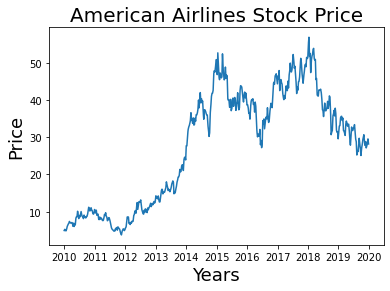
\includegraphics[width=0.45\linewidth]{../img/SeriesAnalysis/American_Serie}
		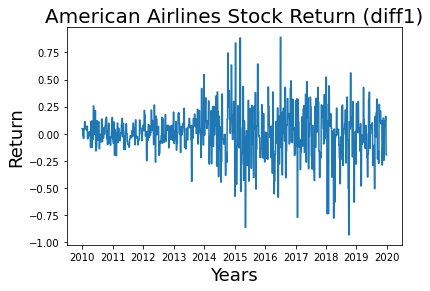
\includegraphics[width=0.45\linewidth]{../img/SeriesAnalysis/American_diffSerie}
		\caption{American Airlines Original Stock Price Series (left) and 1 time differentiated Return Series (right)}
		\label{fig:americanserie}
	\end{figure}
	
	
	Even though the series have different behaviour over time, with respect to the analysis of interest all of them have identical results. With respect to the \textit{NumDiff}, all of the series needed to be discretely differentiated one time to gain stationary behaviour and pass the \textit{ADF Test}. 
	
	Once the analysis is complete, the next step was to implement each of the following methods for time series forecast:
	\begin{enumerate}
		\item ARIMA
		\item ARIMA + GARCH
		\item Random Forest Regressor
		\item Support Vector Machine Regressor
		\item Multi Layer Perceptron Neural Networks
		\item Recurrence Neural Networks
		\item Facebook Prophet Model
	\end{enumerate}
	
	Each of the methods will be briefly explained in the following paragraphs, however the results are clustered together in the end of this section in the tables \ref{table:trainingRMSE} and \ref{table:forecastRMSE}.\\
	
	\textbf{ARIMA and GARCH} \\
	
	The first methods to be implemented are classic linear models for time series forecasting, the Auto Regressive Integrated Moving Average Model and the Generalized Autoregressive Conditional Heteroskedasticity.
	
	The first in constructed with 2 simpler models, the AR (Auto Regressive) and MA (Moving Average), which equations are shown below. This model claims that the present value of the series is linear dependent of the past values until a lag-p in the past as well as in the linear combination of the errors until a lag-q past value. In order to determine the number of past values to use in the model, one can use the Autocorrelation and Partial Autocorrelation Functions, as describer in \cite{tsay2005analysis} and shown below. The \textit{Integrated} part of the name suggests the number of differentiation needed to gain stationary behaviour, since this is a requisite for the model itself.
	
	\begin{equation}
		y_t=\phi_0+\sum_{i=1}^{p}\phi_iry_{t-i}+\alpha_t+\sum_{i=1}^{q}\theta_i\alpha_{t-i}
	\end{equation} 
	
	where $y_t$ is the value of the time series in time step $t$ and $\alpha_t$ is a white noise series.
	
	\begin{figure}[h]
		\centering
		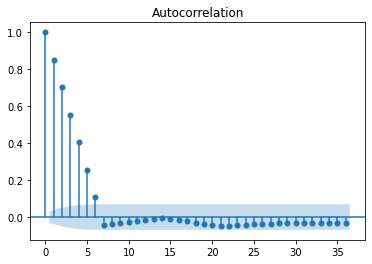
\includegraphics[width=0.45\linewidth]{../img/SeriesAnalysis/ACF_AmericanDiff}
		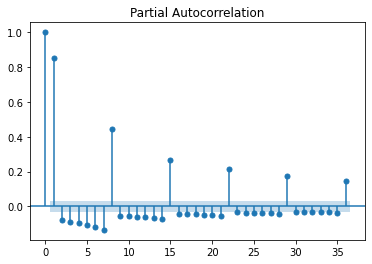
\includegraphics[width=0.45\linewidth]{../img/SeriesAnalysis/PACF_AmericanDiff}
		\caption{ACF and PACF American Airlines Stationary Series}
		\label{fig:acfamericandiff}
	\end{figure}
	
	
	The Garch model is used to describe the volatility (the variance) of the time series and it can integrate the ARIMA model by modeling the $\alpha_t$ white noise (error). The equation that defines a GARCH(m,s) is as follows:
	\begin{equation}
		\alpha_t=\sigma_t\epsilon_t\mbox{,      }\sigma_t^2=\alpha_0+\sum_{i=1}^{m}\alpha_i\alpha_{t-i}^2+\sum_{j=1}^{s}\beta_j\sigma_{t-j}^2
	\end{equation}
	
	\textbf{Random Forests} \\
	
	As known, a Random Forest is an ensemble method implemented with a collection of Decision Trees \cite{bishop2006pattern}. Although known better for classification, Decision Trees, and Random Forest, can be used for regression problems as well.
	
	For a regression problem, each Decision Tree is constructed in a similar way that it would be in a classification problem. Given an tabular input shaped as a \textit{moving window}, each feature is used to determine the best split based on the target value $y_{t+1}$. Once the best splits are determined and the tree is constructed, given a new input, the value of the prediction will be the average of the leaf values this new input reaches. See \cite{decisiontreeregression} and \cite{randomforestregression}.
	
	With respect to the moving window approach, as well as the other input format needed for each model, see the subsection \textbf{Input Formats} in the end of the model's introduction. \\
	
	This model, as well as MLP, SVM AND Prophet were implemented with hyperparameters search. RNN were not because of the long training time and ARIMA/GARCH do not have hyperparameters.\\
	
	\textbf{Support Vector Machines} \\
	
	SVMs for regression are implemented in a analogous way to classification SVMs. The  regressor tries to fit  the best line \textit{hyperplane} within a predefined threshold error value \textit{decision boundaries}. Instead of using the hyperplane to separate different classes, the \textit{SVM Regressor} uses it to fit the behaviour of the time series. See \cite{svmregression}. \\
	
	
	\textbf{Multi Layer Perceptrons}\\
	
	The MLP Networks for regression and classification are implemented and trained in the exact same way. The only difference is that the output layer, instead of being composed of $n$ nodes representing $n$ classes, it is made of a single node, which represents the predicted value $y_{t+1}$ of the series. With that value in hand, the network uses back propagation and gradient descent to find the best weight for its connections, as it is done with a classification network. The input layer is made of the $l$ past values of the series and, for this project, $l=12$.\\
	
	\textbf{Recurrent Neural Networks}\\
	
A recurrent neural network(RNN) is a type of artificial neural network commonly used in speech recognition and natural language processing. Recurrent neural networks recognize data's sequential characteristics and use patterns to predict the next likely scenario. RNNs are distinct from other types of artificial neural networks because they use feedback loops to process a sequence of data that that informs the final output. These feedback loops allow information to persist. \\

The RNN processes the sequence of vectors one by one. While processing, it passes the previous hidden state to the next step of the sequence. The hidden states act as the neural network’s memory, which holds information on previous data the network has seen before. Then the input and previous hidden state are combined to form a vector. The vector then goes through the activation which decides what to do with the data, and the output is the new hidden state.\\

Long short-term memory (LSTM) is an artificial recurrent neural network(RNN) architecture. LSTMs were created as the solution to vanishing gradient problem due to short-term memory. In this project, we used a Vanilla LSTM, which is an LSTM model that has a single hidden layer of LSTM units, and an output layer used to get one prediction value yt+1. The ni is the number of the time steps for one LSTM cell/unit, and nf is the is the number of features which is 1 since we are working with univariate time series. Choosing a right value of ni would avoid you from overfitting with short amount of data and getting explosive predict value. u is the unit number of LSTM and e is the epochs. The bigger the u and e are, and the more data are used to train and fit model. To demonstrate the model, a batch which contains the value of the end of the training data series which has the same length with test series are used to predict the first value in the test series. Then the prediction is added into the end of current batch and also into an array to store all the prediction, and the first value was removed. The batch will be full of predictions, and the information in the batch will be still used to get new predictions until the array was the same length as the test series. Then get the error by comparing the test series and the prediction array. See\cite{abiodun2018state} and \cite{hochreiter1997long}.\\

	
	
	\textbf{Prophet}\\
	
	The Prophet is a Facebook Open Source project for time series predictions based on an additive model that tries to sum together 3 different functions that tries to model trend $g(t)$, seasonality $s(t)$ and holiday/weekend effects $h(t)$. See \cite{taylor2018forecasting} and \cite{prophetwebsite}.
	
	\begin{equation}
		y(t)=g(t)+s(t)+h(t)+\epsilon_t
	\end{equation}
	
	The Trend model, $g(t)$, can be implemented in two different ways, according to \cite{taylor2018forecasting}. First, there is a model that assumes a linear growth over time without a saturation point. Secondly, there is a non linear growth with a carrying capacity as saturation point. The equations that define these models are, respectively:
	
	\begin{align}
		g(t)&=(k+a(t)^T\delta)t+(m+a(t)^T\gamma)\\
		g(t)&=\dfrac{C}{1+exp(-k(t-m))}
	\end{align}
	
	where $k$ is the growth rate, $\delta$ has the rate adjustment, $m$ is the offset parameter, $\gamma$ is a variable to make the function continuous and $C$ is the carrying capacity.
	
	The seasonality model is, basically, a Fourier Series that captures the periodic behaviour of the seasonal model.
	
	\begin{equation}
		s(t)=\sum_{n=1}^{N}\left(\alpha_ncos\left(\dfrac{2\pi nt}{P}\right)+\beta_nsin\left(\dfrac{2\pi nt}{P}\right)\right)
	\end{equation} 
	
	
	At last, the holidays/weekend model is implemented with a auxiliary table that list all the holidays and events. This table is used to add an indicator functions that tells if a time step $t$ occurs during a holiday $i$ and assign a parameter for each holiday which is the corresponding change in the forecast \cite{taylor2018forecasting}. Note that the holiday model is not of large importance for this project since the frequency of the time series is weekly and the table presented above was not implemented.\\ 
	
	\textbf{Input Formats}\\
	
	The models implemented in this project needed two types of input formats, that is, two different ways to reshape the time series in order to implement the algorithms.
	
	First, for \textit{ARIMA}, \textit{GARCH}, \textit{RNN} and \textit{Prophet}, the series were passed as input as the were originally, a pandas series, which is, basically, a list with the values of the series at each time step. Sometimes, instead of a pandas series, a pandas dataframe was needed so that the model had the data of each observation as index.
	
	For \textit{Random Forests}, \textit{SVM} and \textit{MLP} the series were reshaped into a moving window table. That means a original series with the format $[y_{0},y_{1},y_{2},...,y_{t}]$ was reshaped into the following table:
	
	\begin{table}[h]
		\centering
		\begin{tabular}{|llll|l|l|}
			\hline
			\multicolumn{4}{|c|}{Past Steps}                                                                            &  $Y\_\{t\}$ & $Y_{t+1}$ \\ \hline
			\multicolumn{1}{|l|}{$y_{0}$}   & \multicolumn{1}{l|}{$y_{1}$} & \multicolumn{1}{l|}{$y_{2}$}   & $y_{3}$   & $y_{4}$                & $y_{5}$                \\ \hline
			\multicolumn{1}{|l|}{$y_{1}$}   & \multicolumn{1}{l|}{$y_{2}$} & \multicolumn{1}{l|}{$y_{3}$}   & $y_{4}$   & $y_{5}$                & $y_{6}$                \\ \hline
			\multicolumn{1}{|l|}{...}       & \multicolumn{1}{l|}{...}     & \multicolumn{1}{l|}{...}       & ...       & ...                    & ...                    \\ \hline
			\multicolumn{1}{|l|}{$y_{t-5}$} & \multicolumn{1}{l|}{$y_{4}$} & \multicolumn{1}{l|}{$y_{t-3}$} & $y_{t-2}$ & $y_{t-1}$              & $y_{t}$                \\ \hline
		\end{tabular}
	\end{table}
	
	Each row is a window of the time series and the last column will be used as "target" for the supervised learning algorithms. Note that, from row $i$ to row $i+1$ thee window is shifted one unit to the right. The $Y_{t+1}$ column is used as target while the others are passed as features/inputs.\\
	
	\textbf{RMSE Tables}
	
	\begin{table}[h]\label{table:trainingRMSE}
		\centering
		\begin{tabular}{|lll|}
			\hline
			\multicolumn{3}{|c|}{American Series Training RMSE}                                                  \\ \hline
			\multicolumn{1}{|l|}{Method}  & \multicolumn{1}{l|}{Statio} & Non-statio             \\ \hline
			\multicolumn{1}{|l|}{ARIMA}   & \multicolumn{1}{c|}{0.0880}       & \multicolumn{1}{c|}{X} \\ \hline
			\multicolumn{1}{|l|}{GARCH}   & \multicolumn{1}{c|}{0.0880}       & \multicolumn{1}{c|}{X} \\ \hline
			\multicolumn{1}{|l|}{RF}      & \multicolumn{1}{c|}{0.0487}       & \multicolumn{1}{c|}{0.0013}  \\ \hline
			\multicolumn{1}{|l|}{SVM}     & \multicolumn{1}{l|}{0.0609}       & \multicolumn{1}{c|}{0.0725}  \\ \hline
			\multicolumn{1}{|l|}{MLP}     & \multicolumn{1}{l|}{0.0577}       & \multicolumn{1}{c|}{0.0102}  \\ \hline
			\multicolumn{1}{|l|}{RNN}     & \multicolumn{1}{l|}{X}       & \multicolumn{1}{c|}{X}  \\ \hline
			\multicolumn{1}{|l|}{Prophet} & \multicolumn{1}{l|}{0.1253}       & \multicolumn{1}{c|}{0.0431}  \\ \hline
		\end{tabular}
	\end{table}
	
	\begin{table}[h]
		\label{table:forecastRMSE}
		\centering
		\begin{tabular}{|lll|}
			\hline
			\multicolumn{3}{|c|}{American Series Forecasting RMSE}                                                  \\ \hline
			\multicolumn{1}{|l|}{Method}  & \multicolumn{1}{l|}{Statio} & Non-statio             \\ \hline
			\multicolumn{1}{|l|}{ARIMA}   & \multicolumn{1}{c|}{0.1534}       & \multicolumn{1}{c|}{X} \\ \hline
			\multicolumn{1}{|l|}{GARCH}   & \multicolumn{1}{c|}{0.1534}       & \multicolumn{1}{c|}{X} \\ \hline
			\multicolumn{1}{|l|}{RF}      & \multicolumn{1}{c|}{0.0539}       & \multicolumn{1}{c|}{0.0099}  \\ \hline
			\multicolumn{1}{|l|}{SVM}     & \multicolumn{1}{l|}{0.0730}       & \multicolumn{1}{c|}{0.0965}  \\ \hline
			\multicolumn{1}{|l|}{MLP}     & \multicolumn{1}{l|}{0.0648}       & \multicolumn{1}{c|}{0.0050}  \\ \hline
			\multicolumn{1}{|l|}{RNN}     & \multicolumn{1}{l|}{X}       & \multicolumn{1}{c|}{3.7608}  \\ \hline
			\multicolumn{1}{|l|}{Prophet} & \multicolumn{1}{l|}{0.0920}       & \multicolumn{1}{c|}{0.0758}  \\ \hline
		\end{tabular}
	\end{table}
	
	
	%------------------------------------------------------------------------
	\section{Conclusions}
	
	Once the RMSE for all of the models and series are computed and compared, there are, at least, five conclusions one could make:
	\begin{enumerate}
		\item For stationary series, the classic approach produces good results when compared to \textit{machine learning} models
		\item Random Forest produced some of the smallest error rates for all series, stationary or not.
		\item The models for non stationary series produced better errors than the ones for stationary series.
		\item MLP produced the \textbf{best forecast} for all 3 non-stationary series.
		\item The Prophet did not perform well for any of the series.
	\end{enumerate}

	There may be a reason for the results of the Prophet: the series chosen for this project have weekly frequency and do not have the holidays table as well, so the additive model that Prophet implements may not have being adequate for this time series.
	
	The RNN results were specially interesting however, once again there might be a reason: since the hyperparameter search was implemented by \textit{hard coding} for this model and, because of the enormous amount of training time, there is no guarantee that the best, or even a good, choice of hyperparameters was found.
	
	At last, there is enough evidence to answer the main question of this project: \textbf{are Neural Networks the best model for time series forecasting?}. Not necessarily! The MLP has the best results for non stationary series, but the Random Forest displayed comparable RMSE and ARIMA/GARCH, for two of the stationary series, have also shown great errors.
	
	{\small
		\bibliographystyle{cvpr_bibstyle}
		\bibliography{bibliography}
	}
	

	\appendix
	
	
	%-------------------------------------------------------------------------
	
	\section{Helpful Instructions }
	
	This project contains a \textit{README.md} file with \textbf{all} the instructions needed to understand the structure of the project's directories and files.
	
	In order to see the same images for the remaining series, refer to \textit{img directory} in the main directory of this project.
	
	In order to see the all the jupyter notebooks implemented for this project, refer to \textit{code directory} in the main directory of this project.
	
	The \textit{ref directory} has some of the bibliography used during the project and \textit{data directory} has the time series in \textit{csv files}.
	
	\section{Images and Results of remaining Time Series}
	
	This section, although optional for the reader, gives, first, the RMSE Tables for the two remaining time series and the images of all training and forecasts each series.
	
	
	\begin{table}[h]\label{table:usdcadtrainingRMSE}
		\centering
		\begin{tabular}{|lll|}
			\hline
			\multicolumn{3}{|c|}{USD CAD Series Training RMSE}                                                  \\ \hline
			\multicolumn{1}{|l|}{Method}  & \multicolumn{1}{l|}{Statio} & Non-statio             \\ \hline
			\multicolumn{1}{|l|}{ARIMA}   & \multicolumn{1}{c|}{0.0001}       & \multicolumn{1}{c|}{X} \\ \hline
			\multicolumn{1}{|l|}{GARCH}   & \multicolumn{1}{c|}{0.0001}       & \multicolumn{1}{c|}{X} \\ \hline
			\multicolumn{1}{|l|}{RF}      & \multicolumn{1}{c|}{0.0475}       & \multicolumn{1}{c|}{0.0016}  \\ \hline
			\multicolumn{1}{|l|}{SVM}     & \multicolumn{1}{l|}{0.0604}       & \multicolumn{1}{c|}{0.0421}  \\ \hline
			\multicolumn{1}{|l|}{MLP}     & \multicolumn{1}{l|}{0.0548}       & \multicolumn{1}{c|}{0.0088}  \\ \hline
			\multicolumn{1}{|l|}{RNN}     & \multicolumn{1}{l|}{X}       & \multicolumn{1}{c|}{X}  \\ \hline
			\multicolumn{1}{|l|}{Prophet} & \multicolumn{1}{l|}{0.1205}       & \multicolumn{1}{c|}{0.0440}  \\ \hline
		\end{tabular}
	\end{table}
	
	\begin{table}[h]
		\label{table:usdcadforecastRMSE}
		\centering
		\begin{tabular}{|lll|}
			\hline
			\multicolumn{3}{|c|}{USD CAD Series Forecasting RMSE}                                                  \\ \hline
			\multicolumn{1}{|l|}{Method}  & \multicolumn{1}{l|}{Statio} & Non-statio             \\ \hline
			\multicolumn{1}{|l|}{ARIMA}   & \multicolumn{1}{c|}{0.0011}       & \multicolumn{1}{c|}{X} \\ \hline
			\multicolumn{1}{|l|}{GARCH}   & \multicolumn{1}{c|}{0.0011}       & \multicolumn{1}{c|}{X} \\ \hline
			\multicolumn{1}{|l|}{RF}      & \multicolumn{1}{c|}{0.0547}       & \multicolumn{1}{c|}{0.0079}  \\ \hline
			\multicolumn{1}{|l|}{SVM}     & \multicolumn{1}{l|}{0.0586}       & \multicolumn{1}{c|}{0.0463}  \\ \hline
			\multicolumn{1}{|l|}{MLP}     & \multicolumn{1}{l|}{0.0538}       & \multicolumn{1}{c|}{0.0043}  \\ \hline
			\multicolumn{1}{|l|}{RNN}     & \multicolumn{1}{l|}{X}       & \multicolumn{1}{c|}{0.0267}  \\ \hline
			\multicolumn{1}{|l|}{Prophet} & \multicolumn{1}{l|}{0.1004}       & \multicolumn{1}{c|}{0.1302}  \\ \hline
		\end{tabular}
	\end{table}
	
	\begin{table}[h]\label{table:usdbrltrainingRMSE}
		\centering
		\begin{tabular}{|lll|}
			\hline
			\multicolumn{3}{|c|}{USD BRL Series Training RMSE}                                                  \\ \hline
			\multicolumn{1}{|l|}{Method}  & \multicolumn{1}{l|}{Statio} & Non-statio             \\ \hline
			\multicolumn{1}{|l|}{ARIMA}   & \multicolumn{1}{c|}{0.0042}       & \multicolumn{1}{c|}{X} \\ \hline
			\multicolumn{1}{|l|}{GARCH}   & \multicolumn{1}{c|}{0.0042}       & \multicolumn{1}{c|}{X} \\ \hline
			\multicolumn{1}{|l|}{RF}      & \multicolumn{1}{c|}{0.0357}       & \multicolumn{1}{c|}{0.00087}  \\ \hline
			\multicolumn{1}{|l|}{SVM}     & \multicolumn{1}{l|}{0.0448}       & \multicolumn{1}{c|}{0.0734}  \\ \hline
			\multicolumn{1}{|l|}{MLP}     & \multicolumn{1}{l|}{0.0420}       & \multicolumn{1}{c|}{0.0066}  \\ \hline
			\multicolumn{1}{|l|}{RNN}     & \multicolumn{1}{l|}{X}       & \multicolumn{1}{c|}{X}  \\ \hline
			\multicolumn{1}{|l|}{Prophet} & \multicolumn{1}{l|}{0.0895}       & \multicolumn{1}{c|}{0.0377}  \\ \hline
		\end{tabular}
	\end{table}
	
	\begin{table}[h]
		\label{table:usdbrlforecastRMSE}
		\centering
		\begin{tabular}{|lll|}
			\hline
			\multicolumn{3}{|c|}{USD BRL Series Forecasting RMSE}                                                  \\ \hline
			\multicolumn{1}{|l|}{Method}  & \multicolumn{1}{l|}{Statio} & Non-statio             \\ \hline
			\multicolumn{1}{|l|}{ARIMA}   & \multicolumn{1}{c|}{0.0031}       & \multicolumn{1}{c|}{X} \\ \hline
			\multicolumn{1}{|l|}{GARCH}   & \multicolumn{1}{c|}{0.0031}       & \multicolumn{1}{c|}{X} \\ \hline
			\multicolumn{1}{|l|}{RF}      & \multicolumn{1}{c|}{0.0687}       & \multicolumn{1}{c|}{0.0080}  \\ \hline
			\multicolumn{1}{|l|}{SVM}     & \multicolumn{1}{l|}{0.0794}       & \multicolumn{1}{c|}{0.1038}  \\ \hline
			\multicolumn{1}{|l|}{MLP}     & \multicolumn{1}{l|}{0.0863}       & \multicolumn{1}{c|}{0.0063}  \\ \hline
			\multicolumn{1}{|l|}{RNN}     & \multicolumn{1}{l|}{X}       & \multicolumn{1}{c|}{0.0944}  \\ \hline
			\multicolumn{1}{|l|}{Prophet} & \multicolumn{1}{l|}{0.1605}       & \multicolumn{1}{c|}{0.0912}  \\ \hline
		\end{tabular}
	\end{table}
	
	
	\begin{figure}[h]
		\centering
		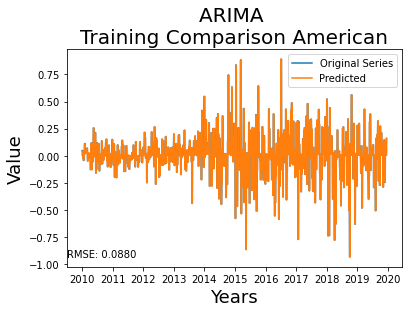
\includegraphics[width=0.45\linewidth]{../img/ARIMA/american_diff_training}
		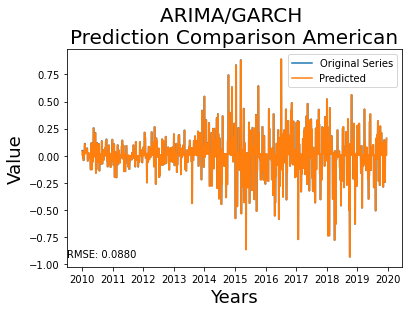
\includegraphics[width=0.45\linewidth]{../img/GARCH/american_diff_training}
		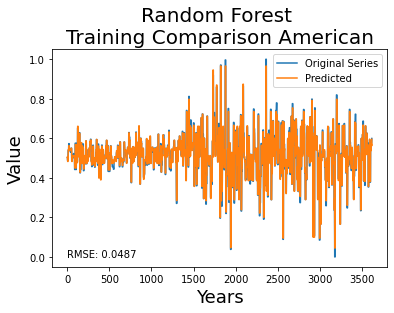
\includegraphics[width=0.45\linewidth]{../img/RandomForest/american_diff_training}
		\includegraphics[width=0.45\linewidth]{../img/SVM/american_diff_training}
		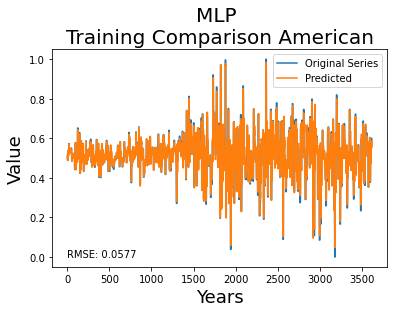
\includegraphics[width=0.45\linewidth]{../img/MLP/american_diff_training}
		%\includegraphics[width=0.45\linewidth]{../img/RNN/american_diff_training}
		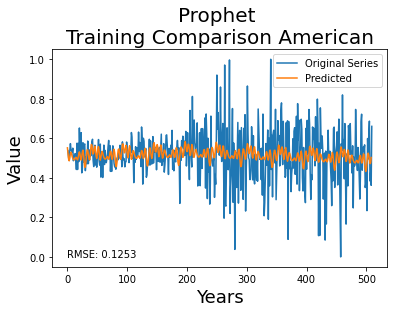
\includegraphics[width=0.45\linewidth]{../img/Prophet/american_diff_training}
		\caption{American Stationary Series Training}
		\label{fig:americandifftraining}
	\end{figure}
	
	\begin{figure}[h]
		\centering
		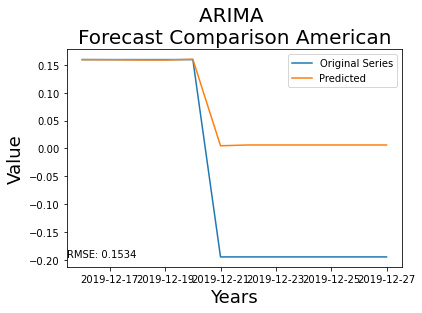
\includegraphics[width=0.45\linewidth]{../img/ARIMA/american_diff_for}
		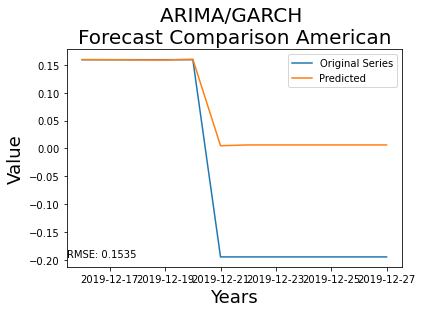
\includegraphics[width=0.45\linewidth]{../img/GARCH/american_diff_for}
		\includegraphics[width=0.45\linewidth]{../img/RandomForest/american_diff_for}
		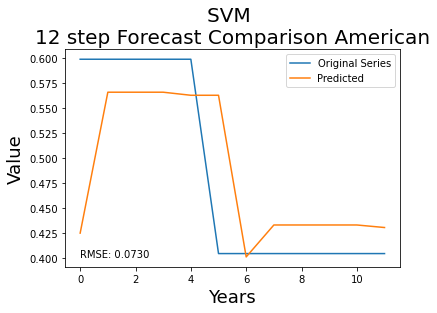
\includegraphics[width=0.45\linewidth]{../img/SVM/american_diff_for}
		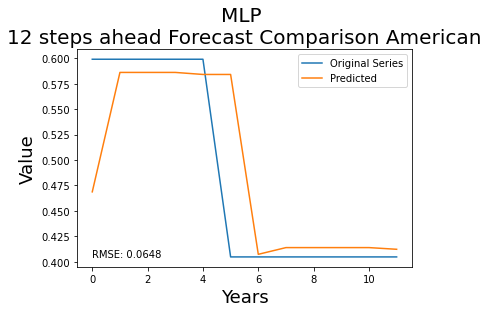
\includegraphics[width=0.45\linewidth]{../img/MLP/american_diff_for}
		%\includegraphics[width=0.45\linewidth]{../img/RNN/american_diff_for}
		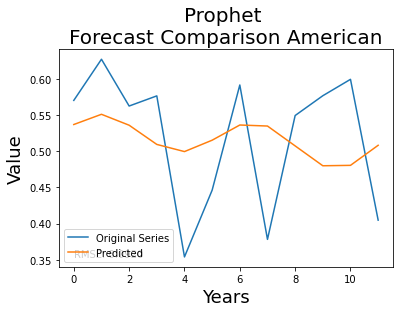
\includegraphics[width=0.45\linewidth]{../img/Prophet/american_diff_for}
		\caption{American Stationary Series Forecast}
		\label{fig:americandiffforecast}
	\end{figure}
	
	\begin{figure}[h]
		\centering
		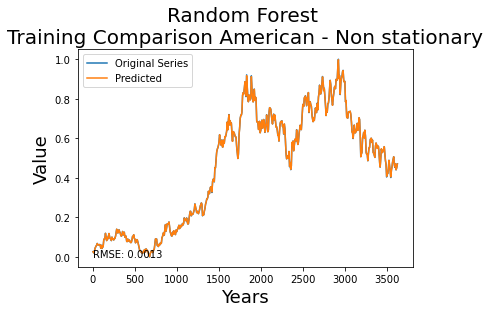
\includegraphics[width=0.45\linewidth]{../img/RandomForest/american_training}
		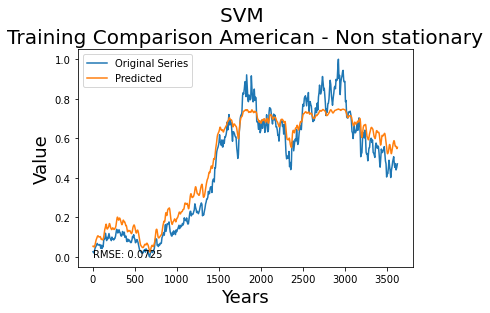
\includegraphics[width=0.45\linewidth]{../img/SVM/american_training}
		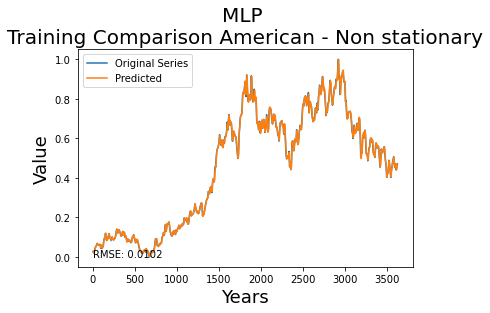
\includegraphics[width=0.45\linewidth]{../img/MLP/american_training}
		%\includegraphics[width=0.45\linewidth]{../img/RNN/american_diff_training}
		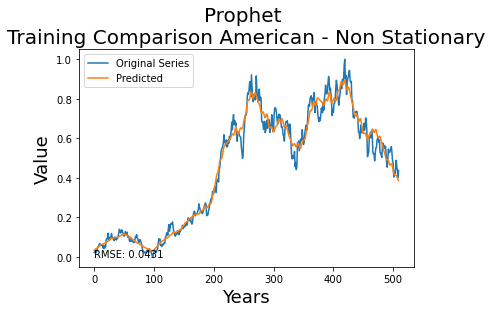
\includegraphics[width=0.45\linewidth]{../img/Prophet/american_training}
		\caption{American Original Series Training}
		\label{fig:americantraining}
	\end{figure}
	
	\begin{figure}[h]
		\centering
		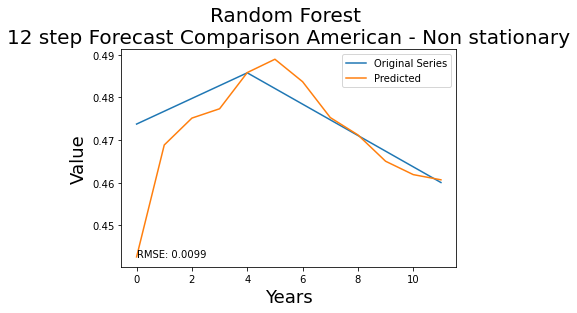
\includegraphics[width=0.45\linewidth]{../img/RandomForest/american_for}
		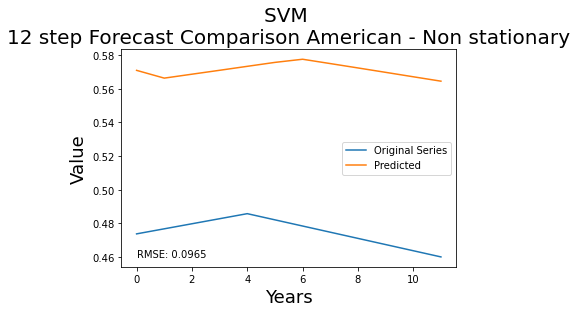
\includegraphics[width=0.45\linewidth]{../img/SVM/american_for}
		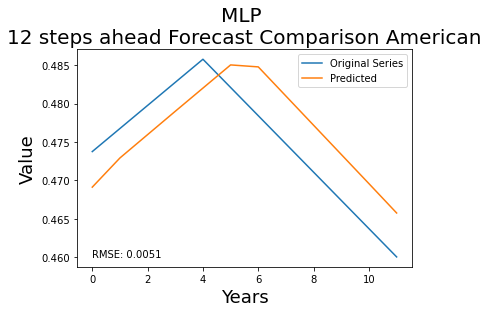
\includegraphics[width=0.45\linewidth]{../img/MLP/american_for}
		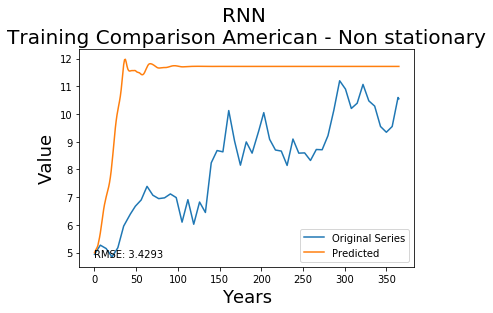
\includegraphics[width=0.45\linewidth]{../img/RNN/american_for}
		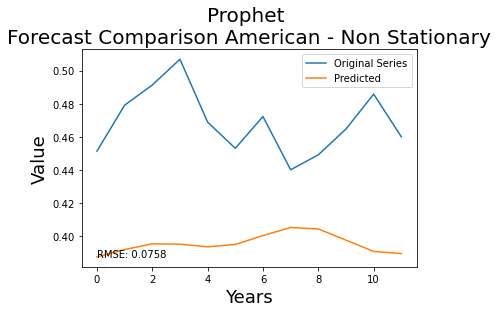
\includegraphics[width=0.45\linewidth]{../img/Prophet/american_for}
		\caption{American Original Series Forecast}
		\label{fig:americanforecast}
	\end{figure}
	

	
	\begin{figure}[h]
		\centering
		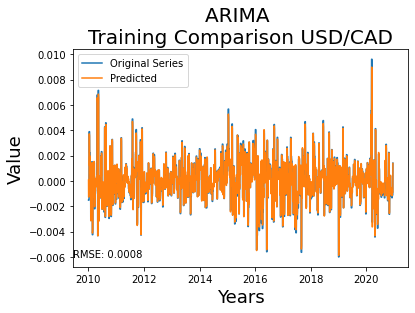
\includegraphics[width=0.45\linewidth]{../img/ARIMA/usd_cad_diff_training}
		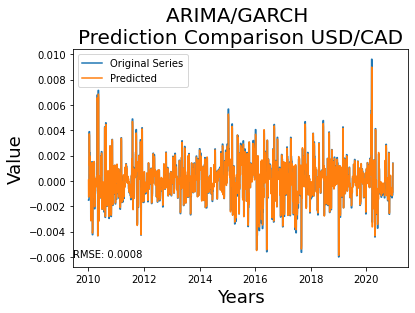
\includegraphics[width=0.45\linewidth]{../img/GARCH/usd_cad_diff_training}
		\includegraphics[width=0.45\linewidth]{../img/RandomForest/usd_cad_diff_training}
		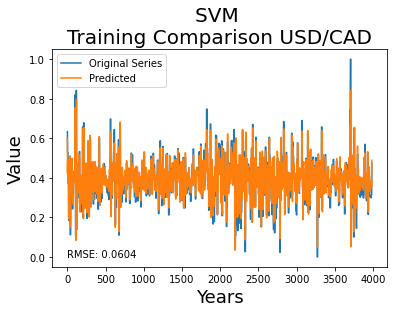
\includegraphics[width=0.45\linewidth]{../img/SVM/usd_cad_diff_training}
		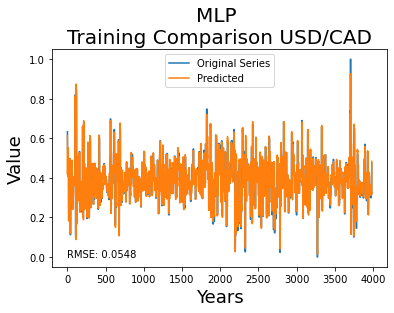
\includegraphics[width=0.45\linewidth]{../img/MLP/usd_cad_diff_training}
		%\includegraphics[width=0.45\linewidth]{../img/RNN/usd_cad_diff_training}
		\includegraphics[width=0.45\linewidth]{../img/Prophet/usd_cad_diff_training}
		\caption{USD/CAD Stationary Series Training}
		\label{fig:usd_caddifftraining}
	\end{figure}
	
	\begin{figure}[h]
		\centering
		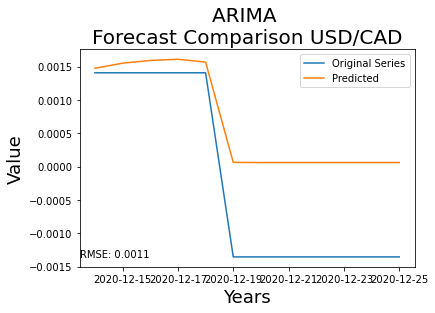
\includegraphics[width=0.45\linewidth]{../img/ARIMA/usd_cad_diff_for}
		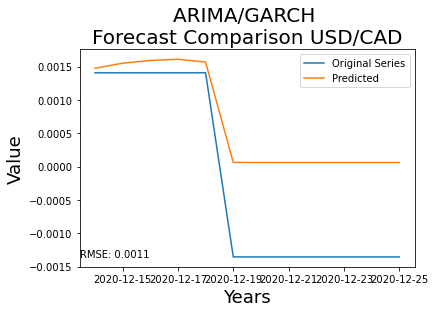
\includegraphics[width=0.45\linewidth]{../img/GARCH/usd_cad_diff_for}
		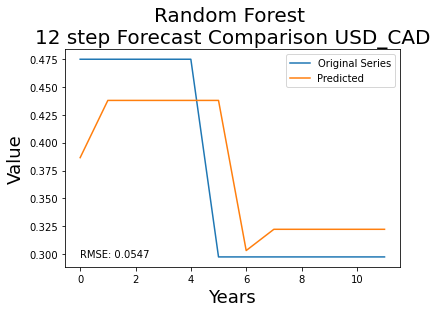
\includegraphics[width=0.45\linewidth]{../img/RandomForest/usd_cad_diff_for}
		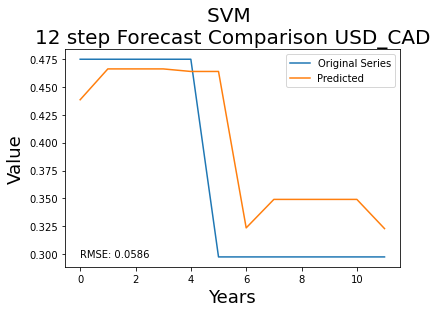
\includegraphics[width=0.45\linewidth]{../img/SVM/usd_cad_diff_for}
		\includegraphics[width=0.45\linewidth]{../img/MLP/usd_cad_diff_for}
		%\includegraphics[width=0.45\linewidth]{../img/RNN/usd_cad_diff_for}
		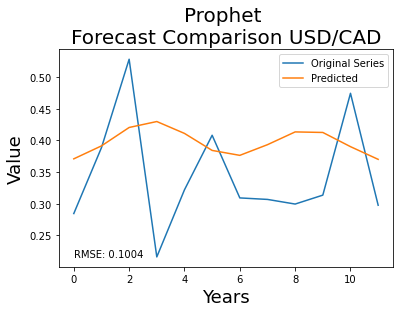
\includegraphics[width=0.45\linewidth]{../img/Prophet/usd_cad_diff_for}
		\caption{USD/CAD Stationary Series Forecast}
		\label{fig:usd_caddiffforecast}
	\end{figure}
	
	\begin{figure}[h]
		\centering
		\includegraphics[width=0.45\linewidth]{../img/RandomForest/usd_cad_training}
		\includegraphics[width=0.45\linewidth]{../img/SVM/usd_cad_training}
		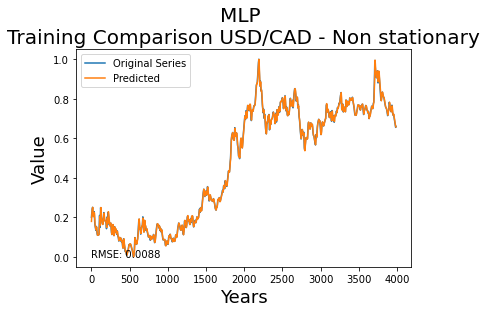
\includegraphics[width=0.45\linewidth]{../img/MLP/usd_cad_training}
		%\includegraphics[width=0.45\linewidth]{../img/RNN/usd_cad_training}
		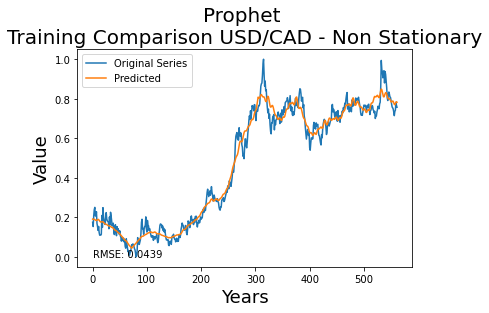
\includegraphics[width=0.45\linewidth]{../img/Prophet/usd_cad_training}
		\caption{USD/CAD Original Series Training}
		\label{fig:usd_cadtraining}
	\end{figure}
	
	\begin{figure}[h]
		\centering
		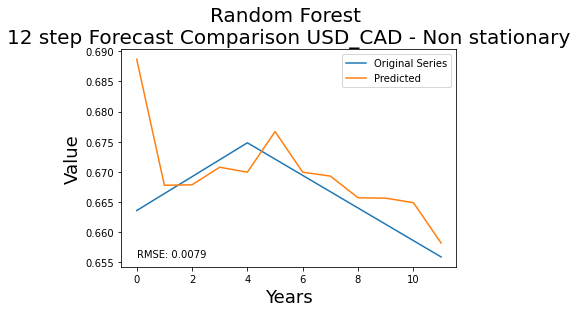
\includegraphics[width=0.45\linewidth]{../img/RandomForest/usd_cad_for}
		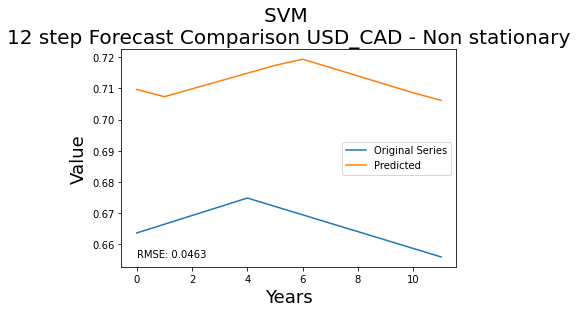
\includegraphics[width=0.45\linewidth]{../img/SVM/usd_cad_for}
		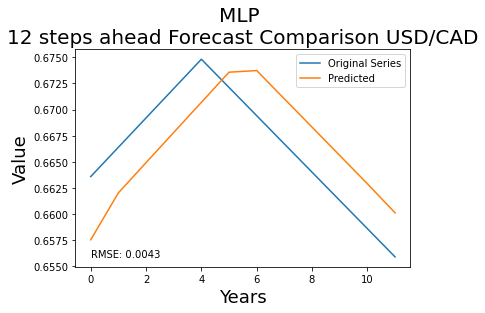
\includegraphics[width=0.45\linewidth]{../img/MLP/usd_cad_for}
		\includegraphics[width=0.45\linewidth]{../img/RNN/usd_cad_for}
		\includegraphics[width=0.45\linewidth]{../img/Prophet/usd_cad_for}
		\caption{USD/CAD Original Series Forecast}
		\label{fig:usd_cadforecast}
	\end{figure}
	
	
	\begin{figure}[h]
		\centering
		\includegraphics[width=0.45\linewidth]{../img/ARIMA/usd_brl_diff_training}
		\includegraphics[width=0.45\linewidth]{../img/GARCH/usd_brl_diff_training}
		\includegraphics[width=0.45\linewidth]{../img/RandomForest/usd_brl_diff_training}
		\includegraphics[width=0.45\linewidth]{../img/SVM/usd_brl_diff_training}
		\includegraphics[width=0.45\linewidth]{../img/MLP/usd_brl_diff_training}
		%\includegraphics[width=0.45\linewidth]{../img/RNN/usd_brl_diff_training}
		\includegraphics[width=0.45\linewidth]{../img/Prophet/usd_brl_diff_training}
		\caption{USD/BRL Stationary Series Training}
		\label{fig:usd_brldifftraining}
	\end{figure}
	
	\begin{figure}[h]
		\centering
		\includegraphics[width=0.45\linewidth]{../img/ARIMA/usd_brl_diff_for}
		\includegraphics[width=0.45\linewidth]{../img/GARCH/usd_brl_diff_for}
		\includegraphics[width=0.45\linewidth]{../img/RandomForest/usd_brl_diff_for}
		\includegraphics[width=0.45\linewidth]{../img/SVM/usd_brl_diff_for}
		\includegraphics[width=0.45\linewidth]{../img/MLP/usd_brl_diff_for}
		%\includegraphics[width=0.45\linewidth]{../img/RNN/usd_brl_diff_for}
		\includegraphics[width=0.45\linewidth]{../img/Prophet/usd_brl_diff_for}
		\caption{USD/BRL Stationary Series Forecast}
		\label{fig:usd_brldiffforecast}
	\end{figure}
	
	\begin{figure}[h]
		\centering
		\includegraphics[width=0.45\linewidth]{../img/RandomForest/usd_brl_training}
		\includegraphics[width=0.45\linewidth]{../img/SVM/usd_brl_training}
		\includegraphics[width=0.45\linewidth]{../img/MLP/usd_brl_training}
		%\includegraphics[width=0.45\linewidth]{../img/RNN/usd_brl_training}
		\includegraphics[width=0.45\linewidth]{../img/Prophet/usd_brl_training}
		\caption{USD/BRL Original Series Training}
		\label{fig:usd_brltraining}
	\end{figure}
	
	\begin{figure}[h]
		\centering
		\includegraphics[width=0.45\linewidth]{../img/RandomForest/usd_brl_for}
		\includegraphics[width=0.45\linewidth]{../img/SVM/usd_brl_for}
		\includegraphics[width=0.45\linewidth]{../img/MLP/usd_brl_for}
		\includegraphics[width=0.45\linewidth]{../img/RNN/usd_brl_for}
		\includegraphics[width=0.45\linewidth]{../img/Prophet/usd_brl_for}
		\caption{USD/BRL Original Series Forecast}
		\label{fig:usd_brlforecast}
	\end{figure}
	%-------------------------------------------------------------------------
	
	
	
	
	
	
	
	
	
	
	
\end{document}
